%%%%%%%%%%%%%%%%%%%%%%%%%%%%%%%%%%%%%%%%%%%%%%%%%%%%%%%%%%%%%%%%%%%%%%
% How to use writeLaTeX: 
%
% You edit the source code here on the left, and the preview on the
% right shows you the result within a few seconds.
%
% Bookmark this page and share the URL with your co-authors. They can
% edit at the same time!
%
% You can upload figures, bibliographies, custom classes and
% styles using the files menu.
%
%%%%%%%%%%%%%%%%%%%%%%%%%%%%%%%%%%%%%%%%%%%%%%%%%%%%%%%%%%%%%%%%%%%%%%

\documentclass[12pt]{article}

\usepackage{sbc-template}
\usepackage{graphicx,url}
\usepackage[brazil]{babel}   
\usepackage[utf8]{inputenc}  
\usepackage{newunicodechar}
\usepackage{float}
\restylefloat{table}
\newunicodechar{²}{\ensuremath{{}^2}}

\sloppy

\title{Predição de Churn em uma base de reclamações \\ utilizando Deep Learning}

\author{Yan Alexander Venera, Anita Maria da Rocha Fernandes, Rodrigo Sant'Ana}

\address{Curso de Especialização em Big Data - Universidade do Vale do Itajaí (UNIVALI) \\
         BR 101, Km 207 (Campus Kobrasol) - 88.102-700 - São José - SC
    \email{yan.venera@edu.univali.br, \{anita.fernandes,rsantana\}@univali.br}
}

\begin{document} 

\maketitle

\begin{abstract}
In this paper, was proposed a unsupervised machine learning application for Churn Prediction using a database with complaints by user to companies, for this, was used an application with deep learning concepts. All complaints database text processing and transforming was reviewed and documented to return a better accuracy for model generation. Sentiment analysis has been used to increment complain text. Lastly has been generated models with accuracy nearby 64\%, this result has been expected when be work with this data to input in machine learning.
\end{abstract}
     
\begin{resumo} 
Neste trabalho, foi proposta a aplicação de aprendizagem de máquina, mais especificadamente, deep learning não supervisionada para detectar o comportamento de Churn em uma base de reclamações feitas por clientes para qual uma empresa. Também é mencionado todos os tratamentos feitos na base de reclamações afim de possuir um resultado mais preciso dos modelos, além do uso da ferramenta de análise de sentimento. Ao final a acurácia dos modelos gerados ficou em torno dos 64\%, um resultado esperado considerando os atributos de entrada da rede.
\end{resumo}

\section{Introdução}\label{sec:into}

Nos dias atuais, onde os dados pessoais são trafegados na internet entre os mais diversos sites que exigem um cadastro prévio para proporcionar uma plataforma de soluções para problemas. Considera-se de interesse das empresas, principalmente aquelas vínculadas a essas plataformas, que cada vez mais se busque conhecer o perfil dos seus clientes. A busca pelo entendimento destes perfis serve de fonte para futuras tomadas de decisões dentro das próprias empresas \cite{tsai:09}. 

Para este fim, a predição de \emph{Churn} é considerada uma métrica comum aplicada no mercado \cite{amin:18} e pode ser resumida dentro deste como a ação em que um cliente deixa de fazer negócios com uma empresa, seja por um cancelamento de contrato, assinatura, ou simplesmente por deixar de consumir produtos/serviços da mesma. Sendo assim, \emph{Churn} pode ser usada em uma empresa como uma forma de gerenciar efetivamente os seus modelos de clientes \cite{coussement:08}.

No Brasil, existem plataformas que fazem o intermédio entre clientes e empresas, proporcionando a interação e ouvidoria entre a percepção dos clientes acerca dos produtos e serviços entregues pelas empresas. Estes ambientes permitem que os clientes possam se queixar de quaisquer problema que possa ter acontecido com algum produto/serviço prestado por uma empresa. Dentro de plataformas na \textit{World Wide Web}, o compartilhamento destas opniões sobre serviços é conhecido como \emph{Eletronic Word-of-Mouth}, em português Boca-a-boca digital \cite{almeida:17}. 

Acredita-se que todos esses dados gerados em plataformas \textit{Web} pelos seus usuários podem maximizar a compreensão sobre comportamentos que não são comuns de serem humanamente perceptíveis. Considera-se também que seja possível extrair características de sentimentos humanos dentro dos textos que são compartilhados. Essa extração de características afim de detectar polaridade de uma sentença, sendo ela positiva ou negativa é conhecida como Análise de Sentimentos \cite{malheiros:13}.

Uma vez que a performance de uma máquina de aprendizado (\textit{Machine Learning}) depende dos métodos escolhidos para sua aplicação juntamente com um tratamento de dados, neste momento, chega-se na área da inteligência artificial chamada de engenharia de recursos. Esta é responsável por representar os dados de maneira prévia conforme conhecimento humano do ambiente e contexto em que os dados estão inseridos, fazendo com que os modelos gerados já tenham um caminho de solução. Entre as diversas maneiras de se representar dados em modelos, nesta pesquisa utiliza-se do que se chama de aprendizagem profunda, ou \emph{deep learning}, que são compostos por transformações não-lineares afim de gerar soluções abstratas \cite{bengio:13}.

Diante do contexto apresentado, esta pesquisa pretente buscar padrões dentro dos textos de reclamações de usuários, dentro de uma plataforma específica para este fim, desconsiderando demais dados pessoais. O textos passaram por tratamentos para que se fosse possível transformá-los em dados onde, geralmente, os modelos de inteligência artificial possuem capacidade analítica e maior acurácia. A partir desses padrões buscou-se obter a probabilidade de predizer quando um determinado usuário tem ou não o comportamento previsto por \emph{Churn}.

\section{Trabalhos Relacionados}\label{sec:related}

Dentro do meio acadêmico é possível relacionar os objetivos de geração de modelos desta pesquisa com trabalhos que relacionam tratamento e compreenção de texto por máquina, a utilização de \emph{deep learning} e demais técnicas de aprendizagem de máquina para inferir a predição de \emph{Churn}, inclusive utilizando dados de reclamações para o mesmo. 

\subsection{Predição de \emph{Churn} baseado em base de reclamações}

Em uma base utilizada para a construção de um modelo preditivo, foram utilizadas informações sobre a reclamação dos clientes e a resposta em forma de reparo da empresa reclamada. Para melhor formatar esses dados, eles foram separados em três grupos, provisões, reclamações e reparos \cite{hadden:06}.

Para criação dos modelos preditivos para a métrica de \emph{Churn} foram utilizadas três técnicas distintas, sendo elas: (a) redes neurais, (b) árvores de decisão, e; (c) regressão linear. Dentre estes modelos, foram foram utilizadas parametrizações estruturais distintas. 

Para as redes neurais, foram aplicadas as arquiteturas \emph{Bayesian} e \emph{Standard} funções diferentes para avaliação do melhor desempenho, porém, todas consistem em duas camadas de processamento e uma camada de saída. Árvores de decisão foram utilizadas para buscar uma saída binária para tradução de um resultado \emph{booleano}. Na regressão linear o método SPSS foi utilizada para calcular o erro padrão de cada uma das vinte e quatro variáveis, depois de uma análise, quatorze delas foram foram levadas em conta para seleção de variáveis. Em todos os modelos foram consideradas sete variáveis de um total de vinte e quatro, escolhidas de acordo uma taxa de erro padrão. 

\begin{table}[H]
\caption{Percentuais de acurácia de \emph{Churn} por modelo} \label{tab:churn_pred}
\begin{tabular}{|c|c|c|c|}
\hline
\textbf{}            & \textbf{Predição de \emph{Churn}} & \textbf{Predição de Não-\emph{Churn}} & \textbf{Acurácia} \\ \hline
Rede Neural \emph{Bayesian} & 70\%                       & 75\%                           & 74\%              \\ \hline
Rede Neural \emph{Standard} & 55\%                       & 79\%                           & 72\%              \\ \hline
Árvore de Decisão    & 66\%                       & 88\%                           & 82\%              \\ \hline
Regressão Linear     & 51\%                       & 94\%                           & 81\%              \\ \hline
\end{tabular}
\end{table}

Conforme os resultados apresentados na tabela \ref{tab:churn_pred}, de maneira geral, as acurácias resultadas obtiveram resultados próximos, entre 72\% e 82\%, é possível verificar que os modelos apresentaram divergências entre acertos de comportamento, ou não comportamento de \emph{Churn}. A árvore de decisão no geral obteve a acurácia maior, juntamente com a regressão linear, porém, as redes neurais foram os modelos que apresentaram maior equilíbrio entre os comportamentos \cite{hadden:06}.

\subsection{\textit{Deep learning} para classificar textos de multiplos rótulos}

O uso de \emph{deep learning} para classificação de textos com um número de respostas maior do que binário foi um dos fatores que levaram esta pesquisa a seguir está técnica de aprendizagem de máquina. Considerando que em bases de dados que exigem uma resposta com complexidade maior do que um binário, o método de \emph{deep learning} obteve acerto de até 96\%. Neste sentido, espera-se que para uma resposta binária, o percentual de acurácia seja similar \cite{liu:17}.

\section{Base de dados}\label{sec:database}

Baseado em padrões de plataformas geradoras de textos e municiada por usuários reais, este trabalho utilizou uma base de dados com cerca de 1,5 milhões de reclamações registradas no site do \emph{ReclameAQUI} entre os anos de 2019 e 2020. É importante citar que apenas o texto da reclamação foi tratado, analisado e usado de base para geração de modelos que pudessem inferir quando uma nova reclamação tendeu ou não ao comportamento de \emph{Churn}.

A base completa contém dados referente à reclamação do cliente, da empresa reclamada e do cliente responsável pela reclamação. Como o objetivo da geração do modelo se limita a processar o texto da reclamação e predizer se o cliente terá ou não o comportamento de \emph{Churn}, foi determinado que as únicas variáveis aleatórias que permaneceriam na base e seriam analisadas neste estudo seriam aquelas vinculadas à reclamação em si e a resposta do cliente sobre voltar ou não voltar a fazer negócios com a empresa, o que entende-se como sendo uma descrição plena do comportamente de \emph{Churn}.

\subsection{Limpeza e tratamento de dados}\label{sec:clean}

A base de dados passou por alguns processos para que pudesse ser utilizada em redes de \emph{deep learning}. Como foi determinado que os dados finais seriam apenas aqueles referentes à reclamação e a estruturação do comportamento de \emph{Churn} ao final do atendimento da reclamação, foram descartados todos os registros da base que não possuiam uma dessas duas variáveis preenchidas obtendo por fim 1.447.890 registros válidos.

O fluxo do processo de limpeza e de tratamento dos texto pode ser visualizado a partir da Figura \ref{fig:fluxo1} abaixo e cada parte deste será tratada com maiores detalhes no decorrer deste documento.

\begin{figure}[ht]
\centering
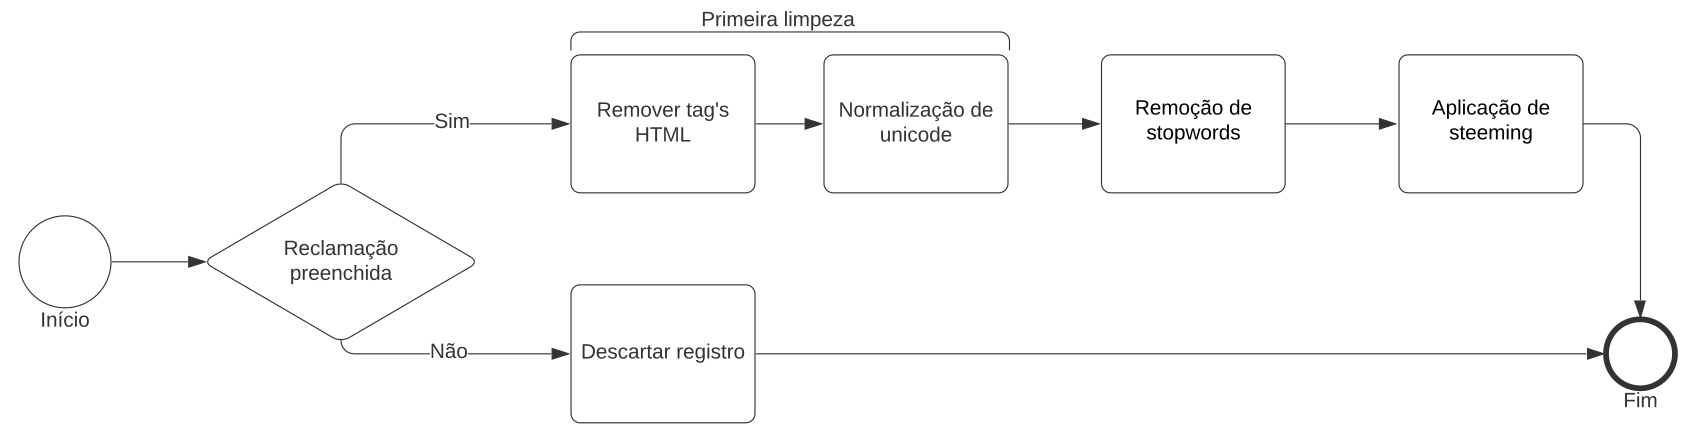
\includegraphics[scale=0.25]{fig/fluxo.png}
\caption{Fluxo de limpeza e tratamento de reclamações}
\label{fig:fluxo1}
\end{figure}

Como os textos da reclamação foram provenientes de uma plataforma on-line, os mesmos possuiam ainda \textit{tags} \emph{HyperText Markup Language} (HTML) em seu corpo, consderando que essas \textit{tags} não possuem correlação com as reclamações, ou seja, não foram dados inseridos pelo usuário em sua reclamação, determinou-se que as tais marcações fossem retiradas do texto. Visando também a normalização de caracteres, remoção de acentuação e caracteres especiais do texto, foi adotada codificação unicode no formato NFKD. Estes dois processos juntos foram marcaram a primeira etapa de limpeza de dados da base. Um exemplo descritivo desta limpeza segue apresentado no próximo parágrafo.

\textbf{Forma de entrada do texto}: ``\emph{\textless{}br /\textgreater{}A empresa fez uma alteração no horário do voo (menos de 2 horas de conexão) e por isso não se pode fazer a marcação de assento.\textless{}br /\textgreater{}Falaram que precisamos ir ao aeroporto no dia e se tiver assento prioritário disponível poderemos utilizá-lo, caso contrário teremos que sentar em qualquer um, mesmo que tenhamos que ficar separados!"}. 

\textbf{Forma de saída do texto}: \emph{``A empresa fez uma alteracao no horario do voo (menos de 2 horas de conexao) e por isso nao se pode fazer a marcacao de assento. Falaram que precisamos ir ao aeroporto no dia e se tiver assento prioritario disponivel poderemos utiliza-lo, caso contrario teremos que sentar em qualquer um, mesmo que tenhamos que ficar separados!"}.

\subsection{Remoção de stopwords}\label{sec:stopwords}

O que é chamado de \emph{stopwords} dentro dos tratamentos de texto para geração de modelos de inteligência artificial, nada mais é do que uma lista de palavras que podem ser removidas de uma sentença, sem que a mesma perca o sentido, dentro desta lista geralmente são considerados principalmente artigos, preposições e conjunções, porém, é comum também considerar dentro das \emph{stopwords} alguns verbos, adverbios e adjetivos, dependendo da linguagem em que se trabalha \cite{mendez:06}. A seguir é apresentado um exemplo de tratamento de texto para remoção de \textit{stopwords}.

\textbf{Forma de entrada do texto}: ``\emph{Tenho o sistema de rastreamento e bloqueio da car system. a meses estou tentando resolver o meu problema. O problema e que nos testes de bloqueio feitos pelo aplicativo, pelo site e pelo telefone nao funcionam.}". 

\textbf{Forma de saída do texto}: ``\emph{Tenho sistema rastreamento bloqueio car system. meses tentando resolver problema. O problema testes bloqueio feitos aplicativo, site telefone nao funcionam.}".

\subsection{Steeming}\label{sec:steeming}

A técnica de \emph{stemming} é consistem combinar / permutar palavras em uma sentença com o intuito de verificar distintas formulações de uma frase com o mesmo sentido e, por sua vez, unificá-las em termos únicos. Esta técnica pode ser chamada também de radical \cite{dias:06}. Desta forma, o tratamento faz com que a palavra dentro da sentença seja substituida pelo seu radical direto, afim de diminuir a quantidade de palavras da base de dados, fazendo com que a vetorização da base seja reduzida também. 

\textbf{Forma de entrada do texto}: ``\emph{Tenho o sistema de rastreamento e bloqueio da car system. a meses estou tentando resolver o meu problema. O problema e que nos testes de bloqueio feitos pelo aplicativo, pelo site e pelo telefone nao funcionam.}". 

\textbf{Forma de saída do texto}: ``\emph{tenh o sistem de rastre e bloquei da car system. a mes est tent resolv o meu problema. o problem e que no test de bloquei feit pel aplicativo, pel sit e pel telefon nao funcion.}".

Para aplicação das abordagens de \emph{steeming} e de \emph{stopwords} foi utilizada as bibliotecas / dicionários nativos em língua portuguesa (pt-br) presentes na ferramenta de \emph{NLTK} para \emph{python}. Todas as palavras foram padronizadas no formato minúsculo, passo importante também para diminuição do número de variações de palavras (e.g. as análises de texto são sensitivas ao caso).

\subsection{Análise de Sentimento}\label{sec:sentiment}

Atualmente, considera-se que, em geral, textos são categorizados em fatos ou opiniões \cite{liu:10}. Desta forma, a partir do tratamento textual de uma reclamação existente na base de dados, espera-se que seja possível determinar a polaridade dos termos utilizados pelo reclamante no momento da da transcrição textual da reclamação.

A ferramenta de análise de sentimento utilizada no presente estudo permitiu a classificação do sentimento de duas formas distintas: 

\begin{itemize}
   \item[a)] Tipo de sentimente detectado (Bom ou Ruim);
   \item[b)] Percentual do tipo de sentiment (Polaridade). 
\end{itemize}

Esta estruturação da resposta da análise de sentimento permitiu um maior detalhamento na geração do modelo de \emph{deep learning}. Para exemplificar a utilização da ferramenta apresenta-se o seguinte caso: considerando o seguinte texto de reclamação do usuário: ``\emph{No dia 01/08 realizei uma compra por telefone nesta loja, além de ser muito mal atendido, o prazo de dois dias não foi cumprido, estou decepcionado com o serviço!}". A seguinte saída é retornada da ferramenta, em formato \emph{JavaScript Object Notation} (JSON): 

\begin{figure}[ht]
\centering
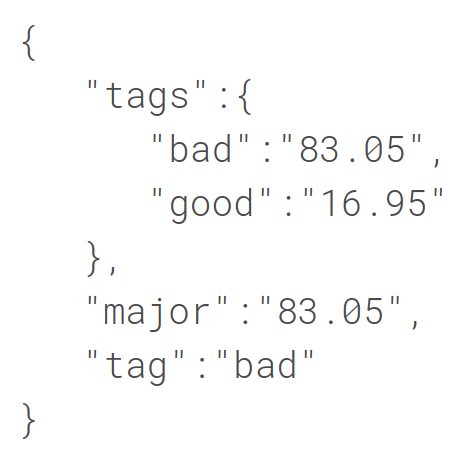
\includegraphics[scale=0.3]{fig/json_sentiment.png}
\caption{Resposta JSON da ferramenta de análise de sentimento}
\label{fig:json_sentiment}
\end{figure}

De acordo com os dados retornados ao término do processo apresentado na Figura \ref{fig:json_sentiment} o que foi preenchido na base foi o sentimento, indicado pelo valor do atributo \emph{tag} e o percentual do sentimento predominante, representado pelo atributo \emph{major}. A ferramenta para utilizada para preenchimento da base com a análise de sentimento, bem como a criação do dicionário de termos para contexto da ferramenta e as demais características da geração dos modelos são de propriedade e responsabilidade da plataforma responsável pela base de dados de reclamações.

\section{Desenvolvimento}\label{sec:develop}

Pretende-se explorar nessa seção a junção de processos de limpeza e tratamento de dados, documentados anteriormente neste documento, juntamente com os processos realizados para que a máquina de aprendizagem possui-se a melhor performance em predizer o comportamento de \emph{Churn} do cliente baseado em sua reclamação.

\subsection{Pré-Processamento de texto}\label{sec:proccess}

Considerando que o classificador de texto pode se comportar de forma melhor depois de passar por certos processos, a abordagem proposta neste projeto passou, necessariamente, pelo fluxo exemplificado na Figura \ref{fig:fluxo2}. 

\begin{figure}[ht]
\centering
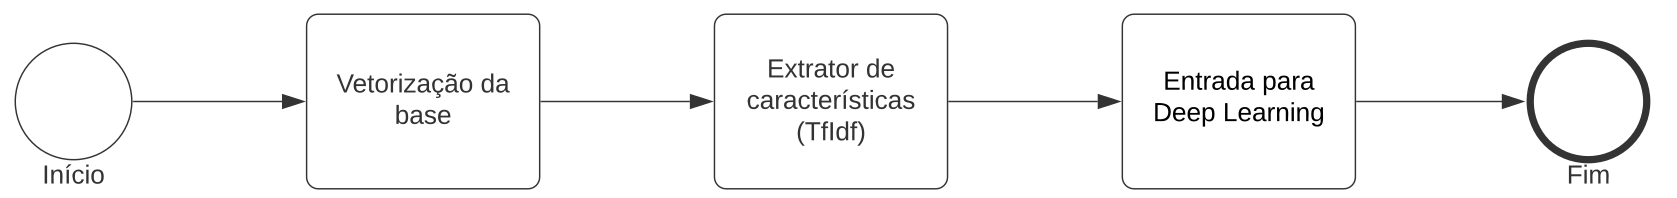
\includegraphics[scale=0.25]{fig/fluxo2.png}
\caption{Fluxo de pré-processamento de texto até a entrada de Deep Learning}
\label{fig:fluxo2}
\end{figure}

Adicionalmente, é importante lembrar que, os dados só podem chegar até esse ponto do processo se não forem descartados pela verificação da Figura \ref{fig:fluxo1}.

\subsubsection{Vetorização}\label{sec:vector}

Uma base de dados de textos, quando totalmente concatenada em apenas uma célula pode ser considerada um único documento de texto \cite{klopotek:03}. Este, entende-se como uma lista de palavras ordenadas afim de fazer sentido. Assim, um documento pode ser representado por um vetor binário, onde o valor de 1 representa que a palavra está contida dentro da lista de palavras presentes neste texto e 0 quando não \cite{ikonomakis:05}.   

Seguindo a vetorização das palavras dentro do texto, o passo seguinte ainda neste método é fazer seleção de características da base, normalmente, está extração é feita de acordo com a frequência com que cada palavra ocorre dentro de uma base \cite{zhang:05}. O resultado da vetorização, geralmente faz com que a base de dados fique simplificada, desta forma, os recursos computacionais para um futuro processamento de dados tendem a serem menores do que quando utilizados os dados puros \cite{ikonomakis:05}.

\subsubsection{Extração de Características}\label{sec:tfidf}

Dentro de um documento de texto, a lista de palavras que compõe este pode ser chamada de vocabulário, ou conjunto de características \cite{ikonomakis:05}, sabendo disso, este processo pretende extrair caracteristicas redundantes e/ou não perceptíveis humanamente.

A ideia de um extrator de características surge na necessidade de indexar documentos e termos na década de 70, o preenchimento de vocabulário com a intenção de quantificar e ordenar a importância de cada item representado no texto foi conhecido como \emph{IDF} \cite{jones:72}, que após a aplicação de uma equação conhece-se por \emph{TF*IDF} \cite{zhang:11}. Nesta pesquisa, o método extrator de características foi proposto com o objetivo de simplificar a quantidade de entradas que uma \emph{deep learning} recebe para trabalhar.

A equação escrita e disposta abaixo, dispõe o tratamento que cada palavra de um documento passa a fim de extrair sua característica dentro do contexto. 

\begin{equation}
W_{ij} = TF_{ij} \times \log \left ( \frac{N}{df_{i}} \right )
\end{equation}

A representação da equação fica da seguinte forma: Wij é o resultado do peso da palavra (representada por i) dentro do documento (representado por j). Enquanto N representa a quantidade de documentos dentro da coleção e TFij representa a frequência em que os termos são apresentados dentro do documento \cite{zhang:11}.

Uma vez que os pesos são atribuidos as palavras do documento, a função do extrator de características passa a ser classificar e ordenar as palavras que tem uma relevância maior dentro da base. Acredita-se que atribuir pesos para as palavrar seja uma maneira mais detalhada de quantificar a representatividade da palavra dentro de uma base de dados \cite{robertson:06}, se comparado a apenas usar o método de vetorização para validar se uma palavra está presente ou não no vocabulário.

\subsection{Divisão da base de dados}\label{sec:proccess}

Depois de realizados todos os tratamentos referentes ao texto, e da aplicação da análise de sentimento, a base de dados foi dividia em dois grupos, o grupo de treinamento e o grupo de teste, eles contaram, respectivamente, com 70\% e 30\% dos dados presentes na base.

\subsection{Deep Learning}\label{sec:deep}

O conceito de \emph{deep learning} pode ser considerado como uma das áreas dentro do que se chama de aprendizagem de máquina, esta, seria a parte de inteligência artificial que trata da máquina adquirir conhecimento a partir de uma base de dados. Vendo desta forma, além do conceito, os algorítmos que formam as ferramentas de aprendizagem de máquina, também se tornam um conjunto de algorítmos fundamentais para a aplicação de deep learning \cite{carrio:17}.

Como outros modelos de aprendizagem de máquina, uma \emph{deep learning} divide-se, na maioria dos casos, em aprendizado supervisionado e não supervisionado. A diferença entre eles é que no primeiro tipo existe uma supervisão de um especialista no contexto em que a base de dados se encontra \cite{deng:13}. No caso deste projeto, como a base de dados não tem uma informação prévia que possa ajudar no aprendizado da máquina, adotou-se o modelo de \emph{deep learning} não supervisionado. 

O arquitetura para geração do modelo desta pesquisa se assemelha com o que encontra-se na literatura especializada com o nome C-LSTM \cite{zhou:15,wang:18,stollenga:15,arbelle:19}. Este surgiu através das junções de uma rede neural convolucional (CNN), sigla do inglês \emph{convolutional neural network} em tradução livre e de uma rede de memorias de termos longos (LSTM), sigla do inglês \emph{long short-term memory network} também em tradução livre \cite{zhou:15}.

A geração de um modelo com arquiteturas e soluções híbridas pretende utilizar as características mais relevantes das duas redes para um acerto maior. Uma rede LSTM tem maior facilidade para aprender um contexto em uma única camada de memória, sem perder informação até o final do treinamento. Já uma rede CNN, tem problemas em manter uma grande quantidade de informação em uma única camada, porém, consegue trabalhar melhor em modelos de múltiplas camadas de treinamento \cite{hassan:17}. Em resumo, dentro desta pesquisa, uma LSTM é responsável pela memória para criação de contextos e uma CNN seria um extrator de caracteristicas do texto.

A geração dos modelos através de \emph{deep learning} foi executada em um servidor da \emph{Amazon Web Services} (AWS) com as seguintes configurações: GPU \emph{NVIDEA Tesla P100} com 16GB de RAM, além de contar com 60GB de RAM. A execução dos \emph{scripts} considerou a criação de 20 modelos distribuidos por épocas, cada época foi responsável pela geração de um modelo juntamente com a avaliação do mesmo por acurácia, o modelo com maior acurácia foi escolhido como modelo final. A partir deste, foram extraídos os dados contidos na seção \ref{sec:result}. Todos os modelos de \emph{deep learning} foram gerados através da ferramenta \emph{Keras}, disponível para programação em \emph{python}.

\subsubsection{Overfitting}\label{sec:overfitting}

Dentro da bibliografia o que chama-se de \emph{overfitting} é o fenômeno onde os modelos gerados em sequência possuem informações suficientes para decorar todas as entradas e saídas de uma base de testes, com isso, considera-se que o modelo não irá mais evoluir, pois nos testes todas as respostas estão corretas e não há substituição de modelo. Este evento acontece geralmente quando são usados, na geração das bases de treinamento, mais termos do que o necessário \cite{hawkins:04}.

\section{Resultados}\label{sec:result}

Os números obtidos nesta seção foram resultantes dos testes feitos executando o modelo gerado na seção \ref{sec:develop} deste documento. A base de testes foi gerada retirando 30\% da base total de dados descritos na seção \ref{sec:database}. 

O modelo gerado obteve um total de 80.670.938 parâmetros disponíveis para treino, esses parâmetros são obtidos através da seguinte lista de camadas do modelo: Incorporação, Quantidade de camadas CNN, Tamanho de LSTM e Densidade. Sendo assim cada, as camadas são definidas da seguinte formas: Incorporação representa a quantidade de palavras contidas no vetor gerado a partir da vetorização de termos. As camadas de CNN são definidas na compilação do modelo, neste caso, foram utilizadas 64 camadas. O tamanho de memória LSTM acompanha o número de camadas de CNN para que informam possam ser geradas e recuperadas em todas as camadas. Por fim, a densidade é o número de saídas possíveis de uma rede, como trata-se de uma rede binária, a densidade é igual a 2. 

Ao final de sua geração, o modelo atingiu de 65\% de acurácia na base de testes. Visando a o aumento do percentual, alguns testes extras foram realizados, tais como: Uso apenas do texto, sem utilização dos dados de análise de sentimento; geração de modelos de redes neurais sem a utilização de \emph{deep learning} com a biblioteca de \emph{sklearn} para \emph{python}; utilização de outros dados presentes na base antes da limpeza (idade, estado e cidade); utilização de outras arquiteturas de \emph{deep learning}, inclusive as que não foram projetadas para saídas binárias. Porém, a geração com maior acurácia foi a que teve todo o seu tratamento descrito neste documento.

A matriz de confusão representada pela tabela \ref{tab:confusion} foi extraída depois da geração do modelo. Nela considera-se que a classe 0 significa que não ocorre o comportamento de \emph{Churn}, e a classe 1 ocorre.

\begin{table}[H]
\centering
\caption{Matriz de confusão resultante do modelo} 
\label{tab:confusion}
\begin{tabular}{|c|c|c|c|}
\hline
\textbf{} & \textbf{0} & \textbf{1} & \textbf{Totais} \\ \hline
\textbf{0} & 62.038 & 104.908 & 166.946 \\ \hline
\textbf{1} & 52.486 & 214.934 & 267.420 \\ \hline
\textbf{Totais} & 114.524 & 319.842 & 434.366 \\ \hline
\end{tabular}
\end{table}

Considerando a tabela \ref{tab:confusion}, a acurácia da classe 0 foi de 37,16\% enquanto a acurácia da classe 1 foi 80,37\%. Com a tabela também é possível calcular a sua sensibilidade, que foi de 54\%, e a sua especificidade de 67\%. A acurácia geral deste modelo foi de 63,76\%.

Durante os testes foi perceptível visualizar que as gerações de modelo atingiam o \emph{overfitting}, descrito na seção \ref{sec:overfitting} deste documento. Dentro do \emph{looping} de épocas da \emph{deep learning}, são separados 20\% dos dados de treinamento para teste do modelo. A partir da terceira época era possível verificar que os modelos já conheciam toda a base de teste, e nesse momento não ocorre mais evolução do mesmo. Este comportamento ocorreu tanto em bases reduzidas como em bases completas.  

\section{Conclusão}\label{sec:conclusion}

A acurácia final de aproximadamente 64\% era um resultado esperado considerando o contexto em que os dados se dispõe, uma geração não supervisionada com textos puros, que por mais que tenham sido tratados, foram feitos por usuários sem nenhum padrão pré-definido, o mesmo apenas se queixou de um atendimento que recebeu de uma empresa, e por fim avaliou o atendimento recebido depois da reclamação. Porém, considera-se que inúmeros os motivos que podem fazer com que uma pessoa tenha ou não o comportamento de \emph{Churn}. 

É possível gerar um tratamento maior apenas para o \emph{overfitting} ocorrido durante as gerações dos modelos, tornar os termos mais enxutos e simplificar a compilação dos modelos de \emph{deep learning} gerados, acredita-se que com o contínuo aprendizado dos modelos, o resultante deve ter um treinamento mais otimizado e em consequência uma acurácia maior.

Esta pesquisa buscou encontrar padrões para o comportamento de \emph{Churn} de um cliente apenas pelos termos utilizados na abertura de uma reclamação, porém, acredita-se que alguns atributos podem enriquecer a base de dados e tornar a acurácia dos modelos maior do que a obtida nesta pesquisa. Dois principais tratamentos são sugeridos: O primeiro deles é a utilização de um perfil de usuário, ou seja, juntar informações pessoais que possam categorizar os usuários em perfis, e o segundo considerar a resposta da empresa a reclamação, tanto a questão de análise de sentimento quanto o tempo em que a empresa levou para dar a resposta, e se o problema do usuário foi realmente resolvido.

\bibliographystyle{sbc}
\bibliography{sbc-template}

\end{document}
